\documentclass[12pt]{article}
\usepackage[utf8]{inputenc}
\usepackage{dirtytalk}
\usepackage{mathrsfs}
\usepackage{blindtext}
\usepackage{csquotes}
\usepackage{mathtools} 	
\usepackage{polynom}
\usepackage{amsthm}
 \usepackage{natbib}
\usepackage[margin=1.8cm ]{geometry}
\usepackage{url}
\usepackage{amssymb,amsmath,graphics}
\title{\textbf{Corrección Parcial 1 Grupos y Anillos}}
\author{
}

\date{\today}

\begin{document}
\renewcommand\qedsymbol{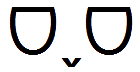
\includegraphics[height=2ex]{Demo_face-removebg-preview.png}}
\maketitle
\begin{enumerate}
    \item En el intervalo $G=(-1,1)$ de la recta real se define la operación:
    $$x\square y=\frac{x+y}{1+x\cdot y}$$
    para $x,y\in G$. Aquí $+$ y $\cdot$ son la suma y multiplicación usual de los números reales. Suponga que la operación $\square$ es cerrada en $G$, demuestre que $(G,\square)$ es un grupo.
    \begin{proof}[\textbf{Demostración:}]
    Para mostrar que $(G,\square)$ es un grupo, como ya tenemos que $\square$ es cerrada falta comprobar que se cumplan las siguientes condiciones:
    \begin{itemize}
        \item La operación $\square$ es asociativa.
        Para mostrar esto consideremos $x,y,z\in G$, luego observe que:
        \begin{align*}
            x\square(y\square z)=x\square\left(\frac{y+z}{1+yz}\right)
                                &=\frac{x+\frac{y+z}{1+yz}}{1+x\left(\frac{y+z}{1+yz}\right)}\\&=\frac{\frac{x+xyz+y+z}{1+yz}}{\frac{1+yz+xy+xz}{1+yz}}\\
                                &=\frac{x+y+z+xyz}{1+xy+xz+yz}\\
                                &=\frac{\frac{x+y+z+xyz}{1+xy}}{\frac{1+xy+xz+yz}{1+xy}}\\
                                &=\frac{\frac{x+y}{1+xy}+\frac{z(1+xy)}{1+xy}}{\frac{1+xy}{1+xy}+\frac{(x+y)z}{1+xy}}\\
                                &=\frac{\frac{x+y}{1+xy}+z}{1+\left(\frac{x+y}{1+xy}\right)z}\\
                                &=\left(\frac{x+y}{1+xy}\right)\square z\\
                                &=(x\square y)\square z
        \end{align*}
        Como mostramos que $x\square(y\square z)=(x\square y)\square z$ podemos asegurar que la operación $\square$ es asociativa.
        \item Existe un elemento $e\in G$ que actúa como neutro. Primero encontremos aquel elemento, este debe cumplir que para $x\in G$ se tiene que $x\square e=x$ luego:
        \begin{align*}
              \frac{x+e}{1+xe}&=x\\
              x+e&=x(1+xe)\\
              x+e&=x+x^2e\\
              0&=x^2e-e\\
              0&=e(x^2-1)
        \end{align*}
        Como $x\in(-1,1)$, $x\neq -1$ y $x\neq 1$ entonces $x^2-1\neq 0$. De esta forma $e=0\in(-1,1)=G$. Ahora note que:
        $$e\square x=0\square x=\frac{0+x}{1+0x}=\frac{x}{1}=x$$
        Así concluimos que si existe un elemento que actúa como neutro ya que para todo $x\in G$ se tiene que:
        $$x\square0=x=0\square x$$
        \item Todo elemento de $G$ tiene inverso. Para hallar ese inverso haremos un análisis similar al que hicimos para hallar el neutro. Tal inverso que llamaremos $x'$ debe cumplir que $x\square x'=0$. Luego:
        \begin{align*}
            \frac{x+x'}{1+xx'}&=0\\
            x+x'&=0\\
            x'&=-x
        \end{align*}
        Claramente $x'=-x\in G$ luego note que:
        $$-x\square x=\frac{-x+x}{1+(-x)(x)}=\frac{0}{1-x^2}=0$$
        De esta manera concluimos que para todo $x\in G$ existe un inverso tal que:
        $$x\square-x=0=-x\square x$$
    \end{itemize}
    De esta forma como hemos mostrado que se cumplen las tres condiciones podemos concluir que $(G,\square)$ es un grupo.
    \end{proof}
    \item (\textbf{V o F}) Sea $G$ un grupo y $a\in G$. Si $a$ es el único elemento de orden $2$, entonces $a$ pertenece al centro de $G$.
    \begin{proof}[\textbf{Verdadero. Demostración:}] Sea $a$ el único elemento de orden $2$ en $G$ es decir:
    $$a^2=e$$
    Donde $e$ es la identidad en $G$. Considere $x\in G$, es evidente que $xax^{-1}\in G$. Observe que:
    \begin{align*}
        (xax^{-1})^2&=(xax^{-1})(xax^{-1})\\
                    &=xa(x^{-1}x)ax^{-1}\\
                    &=xa(e)ax^{-1}\\
                    &=xa^2x^{-1}\\
                    &=xex^{-1}\\
                    &=xx^{-1}=e
    \end{align*}
    Note que como $x$ es arbitrario, se tiene que para todo $x\in G$ el elemento $xax^{-1}$ es de orden $2$ pero por hipótesis $a$ es el único elemento de orden $2$, entonces se debe tener que $xax^{-1}=a$, es decir que para todo $x\in G$, $xa=ax$. De esta forma podemos concluir que $a$ es un elemento del centro de $G$.
    \end{proof}
    \item (\textbf{V o F}) Sea $G$ un grupo y $\varphi:G\to G$ definido por $\varphi(g)=g^{-1}$ para todo $g\in G$. Entonces $\varphi$ es un automorfismo de $G$.
    \begin{proof}[\textbf{Falso. Contraejemplo:}] Considere $G=S_3$. Luego $\varphi:S_3\to S_3$. Consideremos los elementos $\mu_1,\mu_2,\rho_1,\rho_2$ de $S_3$, Primero note que $\rho_1\circ\rho_2=\rho_0$ y que $\mu_1\circ\mu_2=\rho_1$, entonces: 
    $$\rho_2=(\rho_1)^{-1}=\varphi(\rho_1)=\varphi(\mu_1\circ\mu_2)$$
    Ahora observe que $\mu_1\circ\mu_1=\rho_0$ y $\mu_2\circ\mu_2=\rho_0$, entonces:
    $$\rho_1=\mu_1\circ\mu_2=(\mu_1)^{-1}\circ(\mu_2)^{-1}=\varphi(\mu_1)\circ\varphi(\mu_2)$$
    Ahora sabemos que $\rho_2\neq\rho_1$, es decir:
    $$\varphi(\mu_1\circ\mu_2)\neq\varphi(\mu_1)\circ\varphi(\mu_2)$$
    Mostrando de esta forma que $\varphi$ no es un homomorfismo y por tanto no es un automorfismo.
    \end{proof}
    \item (\textbf{V o F}) Sea $G$ un grupo. Si $H\triangle G$ y $G/H$ es cíclico, entonces $G$ es abeliano.
    \begin{proof}[\textbf{Falso. Contraejemplo:}] Considere $G=D_4$ y tomemos $H=\{\rho_0,\rho_1,\rho_2,\rho_3\}$, Note que: 
        $$[D_4:H]=\frac{|D_4|}{|H|}=\frac{8}{4}=2$$
    Entonces $H\triangle D_4$. Ahora observe que:
        $$\left|D_4/H\right|=[D_4:H]=2$$
    Luego como solo hay un grupo de orden $2$, $D_4/H\cong\mathbb{Z}_2$ y por tanto es cíclico. Pero $D_4$ no es abeliano, ya que:
        $$\rho_1\circ\mu_1=\delta_1\neq\delta_2=\mu_1\circ\rho_1$$
    \end{proof}
    \item ¿Cuántos homomorfismos sobreyectivos existen de $S_3$ en $\mathbb{Z}_5$?
    \begin{proof}[\textbf{Cero. Justificación:}] Sea $\phi$ un homomorfismo tal que $\phi:S_3\to\mathbb{Z}_5$. Por el primer teorema fundamental del isomorfismo se tiene que $S_3/\text{ker}\phi\cong \text{Im}\phi$, luego si existiera $\phi$  sobreyectivo se tendría que $\text{Im}\phi=\mathbb{Z}_5$, es decir $S_3/\text{ker}\phi\cong\mathbb{Z}_5$, luego: 
    \begin{align*}
        |S_3/\text{ker}\phi|&=|\mathbb{Z}_5|\\
        \frac{|S_3|}{|\text{ker}\phi|}&=|\mathbb{Z}_5|\\
        \frac{6}{|\text{ker}\phi|}&=5
    \end{align*}
     Para que eso se cumpliera se debería de tener que $|\text{ker}\phi|=\frac{6}{5}$ pero esto es absurdo, entonces no puede existir $\phi$ homomorfismo sobreyectivo.
    \end{proof}
    \item Considere el homomorfismo $\phi:\mathbb{Z}\to\mathbb{Z}_{10}$ definido por $\phi(1)=6$. Encuentre ker$\phi$. Explique.
    \begin{proof}[\textbf{Solución:}]
    Por definición:
    $$\text{ker}\phi=\{n\in\mathbb{Z}:\phi(n)=0\}$$
    Donde ese $0$ representa la clase del cero en $\mathbb{Z}_{10}$. Ahora consideremos los siguientes dos casos:
    \begin{itemize}
        \item $n\geq0$\\
        Observe que tenemos lo siguiente:
            $$\phi(n)=\phi(\underbrace{1+1+\dots+1}_{n\text{ } veces})=\underbrace{\phi(1)+\phi(1)+\dots+\phi(1)}_{n\text{ } veces}=\underbrace{6+6+\dots+6}_{n\text{ }veces}=6n$$
        
        Ahora note que la única forma de que $6n=0$ en $\mathbb{Z}_{10}$ es que $n=5k$ con $k\in\mathbb{Z}^+$ ya que $6n=6(5k)=30k=10(3k)=0$.
        \item $n<0$\\
        Observe que $n=-k$ con $k\in\mathbb{Z}^+$, luego:
        $$\phi(n)=\phi(-k)=-\phi(k)=-(6k)$$
        Por el anterior ítem, $k$ tiene que ser múltiplo de $5$ para que sea $0$ y por tanto $n=-5m$ con $m\in\mathbb{Z}^+$.
    \end{itemize}
    De esto podemos concluir que todos los elementos del kernel son de la forma $5k$ con $k\in\mathbb{Z}$. Concluyendo así que:
    $$\text{ker}\phi=5\mathbb{Z}$$
    \end{proof}
    \item Determine todas las imágenes homomorfas de $D_4$. Explique.
    \begin{proof}[\textbf{Solución:}] $D_4$ tiene tantas imágenes homomorfas como subgrupos normales, entonces miremos cuales son estos subgrupos. Por el teorema de lagrange sabemos que si $H\leq D_4$ entonces $|H|$ divide a $|D_4|=8$, es decir el orden de $H$ es $1,2,4$ o $8$. Luego:
    \begin{itemize}
        \item \textbf{Orden 1: } $H_1=\{\rho_0\}$\\
        Es evidente que $H_1$ es un subgrupo normal de $D_4$. Luego nuestra primer imagen homomorfa es:
        $$\phi_1:D_4\to D_4/H_1$$
        \item \textbf{Orden 2:} Note que hay $5$ elementos de $D_4$ que son de orden dos, luego hay $5$ subgrupos de este orden, veamos cuales de estos son normales:
        \begin{itemize}
            \item $H_2=\{\rho_0,\rho_2\}=\langle\rho_2\rangle$\\
            Basta con probar que las clases laterales son iguales para aquellos elementos que no están en $H_2$.
            \begin{align*}
                \rho_1H_2&=\{\rho_1\circ\rho_0,\rho_1\circ\rho_2\}=\{\rho_1,\rho_3\}=\{\rho_0\circ\rho_1,\rho_2\circ\rho_1\}=H_2\rho_1\\
                \rho_3H_2&=\{\rho_3\circ\rho_0,\rho_3\circ\rho_2\}=\{\rho_3,\rho_1\}=\{\rho_0\circ\rho_3,\rho_2\circ\rho_3\}=H_2\rho_3\\
                \mu_1H_2&=\{\mu_1\circ\rho_0,\mu_1\circ\rho_2\}=\{\mu_1,\mu_2\}=\{\rho_0\circ\mu_1,\rho_2\circ\mu_1\}=H_2\mu_1\\
                \mu_2H_2&=\{\mu_2\circ\rho_0,\mu_2\circ\rho_2\}=\{\mu_2,\mu_1\}=\{\rho_0\circ\mu_2,\rho_2\circ\mu_2\}=H_2\mu_2\\
                \delta_1H_2&=\{\delta_1\circ\rho_0,\delta_1\circ\rho_2\}=\{\delta_1,\delta_2\}=\{\rho_0\circ\delta_1,\rho_2\circ\delta_1\}=H_2\delta_1\\
                \delta_2H_2&=\{\delta_2\circ\rho_0,\delta_2\circ\rho_2\}=\{\delta_2,\delta_1\}=\{\rho_0\circ\delta_2,\rho_2\circ\delta_2\}=H_2\delta_2\\
            \end{align*}
            De esta forma concluimos que $H_2\triangle D_4$ y por tanto nuestra segunda imagen homomorfa es:
            $$\phi_2:D_4\to D_4/H_2$$
            \item $H_3=\{\rho_0,\mu_1\}=\langle\mu_1\rangle$\\
            Observe que:
            $$\rho_1H_3=\{\rho_1\circ\rho_0,\rho_1\circ\mu_1\}=\{\rho_1,\delta_1\}\neq\{\rho_1,\delta_2\}=\{\rho_0\circ\rho_1,\mu_1\circ\rho_1\}=H_3\rho_1$$
            Por lo que $H_3$ no es normal.
            \item $H_4=\{\rho_0,\mu_2\}=\langle\mu_2\rangle$\\
            Observe que:
            $$\rho_1H_4=\{\rho_1\circ\rho_0,\rho_1\circ\mu_2\}=\{\rho_1,\delta_2\}\neq\{\rho_1,\delta_1\}=\{\rho_0\circ\rho_1,\mu_2\circ\rho_1\}=H_3\rho_1$$
            Por lo que $H_4$ no es normal.
            \item $H_5=\{\rho_0,\delta_1\}=\langle\delta_1\rangle$\\
            Observe que:
            $$\rho_1H_5=\{\rho_1\circ\rho_0,\rho_1\circ\delta_1\}=\{\rho_1,\mu_2\}\neq\{\rho_1,\mu_1\}=\{\rho_0\circ\rho_1,\delta_1\circ\rho_1\}=H_5\rho_1$$
            Por lo que $H_5$ no es normal.
             \item $H_6=\{\rho_0,\delta_2\}=\langle\delta_2\rangle$\\
            Observe que:
            $$\rho_1H_6=\{\rho_1\circ\rho_0,\rho_1\circ\delta_2\}=\{\rho_1,\mu_1\}\neq\{\rho_1,\mu_2\}=\{\rho_0\circ\rho_1,\delta_2\circ\rho_1\}=H_6\rho_1$$
            Por lo que $H_6$ no es normal.
        \end{itemize}
        De esta forma terminamos los subgrupos de orden $2$.
        \item \textbf{Orden 4:} Primero notemos que todo subgrupo de orden $4$ es normal, ya que:
        $$[D_4:H]=\frac{|D_4|}{|H|}=\frac{8}{4}=2$$
        y por la propiedad del índice ese $H$ es normal, luego existen tres subgrupos de orden $4$, que son:
        \begin{itemize}
            \item $H_7=\{\rho_0,\rho_1,\rho_2,\rho_3\}=\langle\rho_1\rangle=\langle\rho_3\rangle$
            \item $H_8=\{\rho_0,\rho_2,\mu_1,\mu_2\}=\langle\{\rho_2,\mu_1\}\rangle=\langle\{\rho_2,\mu_2\}\rangle$
            \item $H_9=\{\rho_0,\rho_2,\delta_1,\delta_2\}=\langle\{\rho_2,\delta_1\}\rangle=\langle\{\rho_2,\delta_2\}\rangle$
        \end{itemize}
        Por lo tanto tenemos tres imagenes homomorfas mas, que son:
        \begin{align*}
           \phi_3:D_4\to D_4/H_7\\
           \phi_4:D_4\to D_4/H_8\\
           \phi_5:D_4\to D_4/H_9
        \end{align*}
        \item \textbf{Orden 8:} Por ultimo tenemos el otro subgrupo trivial que es $H_{10}=D_4$ que es también evidente que es normal en si mismo, luego nuestra sexta y ultima imagen homomorfa es:
        $$\phi_6:D_4\to D_4/D_4$$
    \end{itemize}    
    \end{proof}
    \item Sea $G$ un grupo con centro $Z:=Z(G)=\{x\in G | xa=ax \forall a\in G\}$. Pruebe que si el grupo cociente $G/Z$ es cíclico entonces $G$ es abeliano.
    \begin{proof}[\textbf{Demostración:}] Como $G/Z$ es cíclico, quiere decir que $G/Z=\langle kZ\rangle$ con $k\in G$. Ahora consideremos $x,y\in G$, luego podemos construir las clases laterales $xZ,yZ\in G/Z=\langle kZ\rangle$ es decir que $xZ=(kZ)^n$ y $yZ=(kZ)^m$ para algunos $n,m\in\mathbb{Z}$. Note que por definición de normalidad $(kZ)^n=k^nZ$ y $(kZ)^m=k^mZ$. Ahora consideremos $e\in G$ como la identidad, es evidente que $e\in Z$ por definición de el elemento identidad, luego note que:
    \begin{align*}
        x&=xe\in xZ=k^nZ\\
        y&=ye\in yZ=k^mZ
    \end{align*}
    Eso quiere decir que $x=k^nz_1$ y $y=k^mz_2$ para algunos $z_1,z_2\in Z$. Entonces:
    \begin{align*}
        xy&=(k^nz_1)(k^mz_2)\\
          &=k^n(z_1k^m)z_2\\
          &=k^n(k^mz_1)z_2\\
          &=(k^nk^m)(z_1z_2)\\
          &=k^{n+m}(z_2z_1)\\
          &=k^{m+n}(z_2z_1)\\
          &=(k^mk^n)(z_2z_1)\\
          &=k^m(k^nz_2)z_1\\
          &=k^m(z_2k^n)z_1\\
          &=(k^mz_2)(k^nz_1)=yx
    \end{align*}
    Note que todas estas manipulaciones son posibles ya que $z_1,z_2\in Z$, es decir que conmutan con todos los elementos de $G$, en particular con $k^n$ y $k^m$. De esta forma como para $x,y\in G$ arbitrarios, mostramos que $xy=yx$ podemos concluir que $G$ es abeliano.
        
    \end{proof}
\end{enumerate}





\end{document}
